\documentclass[iop]{emulateapj}
\usepackage{color,graphicx,hyperref,natbib}
\graphicspath{{figures/}}

\newcommand{\blue}{\color{blue}}
\newcommand{\tam}{\color{blue}}
\newcommand{\tamcom}{\color{red}}
\newcommand{\red}{\color{red}}
\newcommand{\orange}{\color{orange}}
\newcommand{\purple}{\color{purple}}
\newcommand{\green}{\color{LimeGreen}}
\newcommand{\myemail}{samuelreay@gmail.com}
\newcommand{\runz}{\textsc{Runz}}
\newcommand{\thesisname}{\textsc{Marz}}

\shorttitle{Manual and Automatic Redshifting Software}
\shortauthors{S. R. Hinton}


\begin{document}

\title{\thesisname{}: Manual and Automatic Redshifting Software}

\author{S. R. Hinton, T. M. Davis}
\affil{Department of Physics, The University of Queensland, Brisbane, QLD 4072, Australia}
\affil{ARC Centre of Excellence for All-sky Astrophysics (CAASTRO)}

\begin{abstract}
{\tam The Australian Dark Energy Survey (OzDES) is a 100-night spectroscopic survey underway on the Anglo-Australian Telescope using the fibre-fed 2-degree-field (2dF) spectrograph.  We have developed a new} redshifting application \thesisname{} {\tam with greater usability, flexibility, and wider range of object types than} the \runz{} software package {\tam previously used for redshifting spectra from 2dF.}  \thesisname{} is an open-source, client-based web-application which provides an intuitive interface and powerful automatic matching capabilities to consume FITs files generated from the AAOmega spectrograph and produce high quality spectroscopic measurements.  Behind the scenes, a cross-correlation algorithm is used to match input spectra against a variety of stellar and galactic templates, and automatic matching performance for high quality spectra has increased from 57\% (\runz{}) to 94\% (\thesisname{}). Spectra not matched correctly by the automatic algorithm can be easily redshifted {\tam manually} by cycling automatic results, manual template comparison, or marking spectral features.
\end{abstract}

\section{Introduction}

{\tamcom Introduce what redshifting is first, and motivate the need for the software by explaining what OzDES requires ... i.e. more object types than previous surveys, many users and therefore need for easy installation, wider redshift range than previous surveys...}
 
A variety of redshifting solutions have been developed in the past, with much of the developed software being spectrograph or survey specific. The OzDES team has previously relied on a version of the \runz{} software package, modified for use in the WiggleZ survey, and it is against this modified version of \runz{} that we compared results to in this report. Unfortunately, the legacy nature of the code makes installation and usage overly difficult for members of the team, and the low performance of the automatic matching algorithms within \runz{} for both low signal-to-noise and high-redshift data has prompted the development of a modern software replacement.\\

{\tamcom Outline the requirements of the redshifting software.  What does the survey need?  The rest of the paper will explain how you achieved these goals. }

\section{Platform}

The choice of utilising a browser platform by implementing the matching software as a web application allows access to the software from any laptop or desktop with an internet connection. The interface utilises Google's AngularJS framework and HTML5's Web Worker API for multi-threaded processing, along with Twitter's Bootstrap via Angular UI's Bootstrap components to allow for rapid UI development and prototyping with minimal code boilerplate and reimplementation of common tasks. Communication to Web Workers and any future potential server communication uses JSON format, and will conform to the REST interface. Utilisation of local storage has the benefit that results are not lost when exiting the application or refreshing the browser, negating one of the major disadvantages of stateful web applications. Settings changes are persisted via setting cookie properties instead of using local storage.\\

The code base for \thesisname{} is hosted publically on GitHub\footnote{\url{https://github.com/Samreay/Marz}}, allowing for open issue management, feature requests, open collaboration, forking of the project and instant web-hosting\footnote{\thesisname{} can be found at \url{http://samreay.github.io/Marz/}}.



\section{Matching Algorithm}

{\tam The algorithm that takes an observed spectrum and measures the redshift is the heart of any redshifting program.}
The matching algorithms in \thesisname{} utilise a modified version of the AutoZ algorithm implemented by Ivan Baldry \citep{baldry2014galaxy}. FITs {\tamcom pretty sure it's just FITS} file input from the AAOmega spectrograph undergo two distinct steps of processing: (1) the preprocessing stage to clean the data and (2) the matching process {\tam to align the observed spectra with template spectra, simultaneously finding the best-fit object type and shifting it to the best-fit redshift}.\\

The preprocessing stage is designed to remove any bad pixels and cosmic rays from the data before being returned back to the interface, so that the user can manually redshift using the cleaned data. 
\begin{itemize}
\item {\bf Bad pixels} are defined when the intensity spectrum is not a number, negative or exceeds a certain threshold, or if the variance spectrum for the pixel is negative. 
\item {\bf Cosmic rays} are identified via neighbouring pixels exceeding thirty standard deviations from the mean.
\end{itemize}
Both bad pixels and cosmic rays are replaced with a mean of four and two pixels to either side respectively. 

{\tamcom  Explain why continuum subtraction is a necessary step.}

Continuum is initially subtracted via the method of rejected polynomial subtraction, where a polynomial is iteratively fitted to the spectrum and all points greater than 3.5 standard deviations from the mean are removed from the fitting process. {\tamcom When does this process stop?}  

The matching process takes the output of the preprocessing step in the form of an intensity spectrum and a variance spectrum, and first duplicates the intensity spectrum so that two copies exist internally. This is {\tam necessary because} the matching of the broad-featured quasar template differs to matching of the other templates, and the copy of the intensity spectrum used for quasar matching shall now be referred to as the quasar spectrum, and the other spectrum - used to match all other templates, shall be referred to as the general spectrum. 

{\tam Both spectra are better matched to template spectra after they have gone through a smoothing process to reduce noise.}  The quasar spectrum undergoes smoothing via a rolling-point exponential decay mean function of 7 pixel window, with exponential decay factor of $0.9$. Instead of smoothing, the general spectrum undergoes a second step of continuum subtraction, where a boxcar smoothed median filter (121 pixel window of boxcar smoothing and 51 pixel window median filter) is subtracted from the spectrum. 

The general spectrum then has error adjustment applied, where the variance is set to a maximum of its original value or the nearest neighbour. {\tamcom Explain this previous statement.  Not clear.   Also include something about "why this is necessary". }  The variance spectrum is then widened again, where each pixel is set to a maximum of its original value or 70\% of a thirteen pixel median filter of width 13 pixels. The intensity of the general spectrum is divided by the variance spectrum to down-weight pixels with higher uncertainty. As we wish to preserve broad features found in quasar spectra, the quasar error adjustment process is different. A median filter of 81 pixel width is applied, and then the result is smoothed with boxcar smoothing using a window of 25 pixels. In order to preserve even more broad shape, the variance of the spectrum is increased by addition of twenty times the minimum spectrum variance. The quasar intensity is then divided by the adjusted variance to produce a spectrum that retains broad features and shapes, but down weights sections of higher variance which are commonly found at wavelengths close the ends of the spectroscopic CCD range.

{\tamcom Again we need a "why" here.  What does this step achieve?}
Both the general and the quasar spectrum undergo cosine tapering and root-mean-square normalisation, before being oversampled and Fourier transformed. The quasar spectrum's transformation is then cross correlated with the quasar template, and all other templates are cross correlated with the general spectrum. Cross correlation results are then inverse transformed and peaks within allowed redshift ranges are selected. If prior information on the object type is accessible in the FITs file, the peaks for each template are then weighted. Peaks from all templates are then sorted together, and the highest {\tam correlation} templates have a quadratic fit applied around the peak (for sub-pixel determination of local maxima) before being returned to the user as the results of the matching process {\tam -- that is, a redshift.} 

{\tamcom You haven't mentioned redshifting much during this description (only in the "peaks within allowed redshift ranges" comment.  Explain or emphasise that this is where the actual redshifting is done.  Also, can you make a figure with an example cross-correlation spectrum, compared to the real spectrum shifted to two different cross-correlation peaks and compared to a template?  (I can explain this in person.)}



\begin{figure}
\centering
\includegraphics[width=\columnwidth]{2dfComp.png}
\caption{A comparison of matching efficiency using high signal-to-noise data from the 2dFLenS survey and a matching threshold of $\delta z \leq 0.01$. 2217 QOP4 spectra from ten fields are compared in this plot. The vertical axes shows the redshift assigned by an experienced redshifter, and is taken to be correct in this comparison. The horizontal axes show the automatic results of the four algorithms being compared: the \runz{} cross correlation algorithm, the \runz{} emission line matching algorithm, Autoz and Marz. The total accuracy of the algorithms is detailed in the legend. The \thesisname{} algorithm and Autoz offer comparable accuracy for high redshift spectra, with Autoz pulling ahead slightly due to an increased number of templates being used in the matching process.}
\label{fig:high}
\end{figure}


\begin{figure}
\centering
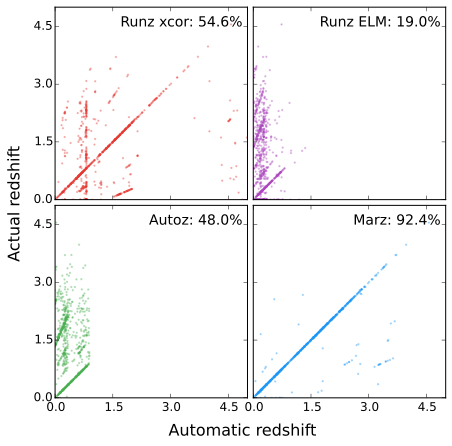
\includegraphics[width=\columnwidth]{run009Comp.png}
\caption{Low signal-to-noise, high-redshift data from the OzDES survey is used in this comparison of matching capability, with a redshift threshold of $\delta z \leq 0.01$. 1083 spectra from eight fields with a redshift range of up to 4.55 are used in this comparison. \runz{} emission line matching performs the worst, with strong diagonal lines of non-unity slope showing repeated spectra feature misidentification. Vertical banding in the \runz{} cross correlation algorithm significantly impacts its effectiveness, and Autoz's lack of high redshift templates and hard-coded $z=0.9$ cutoff make the comparison almost inapplicable. Here the quasar specific matching algorithm used by \thesisname{} stands out, giving a success rate of over 90\% for quasar spectra.}
\label{fig:low}
\end{figure}





\section{Matching Performance}

Performance testing for \thesisname{} was conducted by looking at two sets of distinct data - one from the OzDES team with low signal-to-noise data at high redshift, and one from the 2dFLenS team with high signal-to-noise data. {\tamcom Make sure you describe 2dFLenS in the intro as well.} In both cases, manual redshifting was performed by experienced redshifters in \runz{}, and the automatic matches produced by \runz{} and the automatic results returned by \thesisname{} were compared to the manually assigned redshift for all results assigned a QOP of 4 (99\% confidence interval). Comparisons were also made with the Autoz program, {\tam which is the software being used for the GAMA survey and also being adopted by the 2dFLenS team.  These surveys have a smaller number of object types  and smaller redshift ranges than OzDES, and therefore have simpler requirements for the redshifting software}. These high and low signal-to-noise results are shown in Figures \ref{fig:high} and \ref{fig:low}. The redshifting accuracy of \thesisname{} for high signal-to-noise data gave the correct redshift for 97.5\% of QOP4 spectra, a failure rate far less than that offered by \runz{} and comparable to Autoz. For the low signal-to-noise (high redshift) OzDES data, the accuracy of \thesisname{} was $\approx 92$\%. This is in comparison to the best \runz{} algorithm giving a total accuracy of 54.6\%.  {\tamcom What about Autoz?}

In addition to this, a normalised probability distribution of likelihood for spectral line misclassification can been produced by combining the high and low signal-to-noise data, where the probability for a misclassification per correct classification can be inspected. This has been done for QOP 4 and QOP 3 (90\% confidence) results, in Figure \ref{fig:f4}. Commonly misidentified {\tam spectral} lines are labelled in the figure, and can be seen to be a primary source of misclassification across all algorithms. The common [O$_{\mathrm{II}}$]/[O$_{\mathrm{III}}$] misclassification is strongly present in the \thesisname{} failure rates, however its significance drops to approximately 10\% of the total failure rate when only QOP4 misclassifications are considered, with the majority of the total failure rate of 4.1\% centered around 1. Whilst the expected failure rate for QOP 3 redshifts is ten times higher than for QOP 4 values, this still warrants extra investigation and potential down weighting of high redshift O$_{\rm{II}}$ matches. Commonly misclassified features are also visible on Figure \ref{fig:high} and \ref{fig:low} as linear relationships off the diagonal.








\begin{figure}[h]
\centering
\includegraphics[width=\columnwidth]{errorRateqop3.png}
\caption{The percentage chance, per successfully assigned redshift of quality 3 or 4, of assigning an incorrect redshift $z_A$ with respect to correct manual redshift $z_M$. Peaks in the probability distribution generally represent misidentified spectral lines, and common misidentification ratios have had the corresponding spectral lines labelled, such that the first label, MgII/H$\alpha$ represents the MgII feature misidentified as H$\alpha$ instead. Performance for \runz{} cross correlation, \runz{} emission line matching, Autoz and \thesisname{} are shown respectively in panels (a), (b), (c) and (d). Panel probability axes are not scale with one another, and the area covered represents the total failure rate. The 2dFLenS and OzDES data from Figures \ref{fig:low} and \ref{fig:high} are combined in this analysis, and QOP3 spectra (90\% confidence interval) have been included to give a greater number of sample points. The high relative failure rate of \thesisname{} around 1 are due to broad line matches which are not as well constrained as emission line spectrum. The total failure rates are given as follows: \runz{} cross correlation: 37.5\%, \runz{} emission line matching: 71.0\% failure rate, Autoz: 18.6\% failure rate, \thesisname{}: 6.9\% failure rate.}
\label{fig:f4}
\end{figure}






\begin{figure*}[H]
\centering
\includegraphics[width=\textwidth]{InterfaceZ.png}
\caption{The overview screen, showing data from a FITs file courtesy of Chris Blake and the 2dFLenS survey. Users can switch between a sortable tabular view and a graphic tile view, filter on object types, redshift ranges, templates and QOP values. The top of the screen shows the navigation menu, file completion progress bar and input for user initials. Visible at the bottom of the screen is the application footer, which shows the program's progress through automatic matching (automatically matched templates are shown in red in the graphical tiles). The bar changes colour depending on progress - green for preprocessing, red for matching and blue for completed. During the first two stages, a pause button is available to the user. If any results exist, a download button is available, which saves the current results to the file system.}
\label{fig:overview}
\end{figure*}

\begin{figure*}[H]
\centering
\includegraphics[width=\textwidth]{InterfaceZ2.png}
\caption{The detailed matching screen, showing spectrum 7 seen in the Overview screen in Figure \ref{fig:overview}. The menus at the top of the page allow the user to toggle data on or off (variance, sky spectrum, templates and whether to use the raw data or processed data). The menu bar also allows the user to reset to automatic or manual results, smooth the data, select which template to compare against, toggle between the best five automatic results, change the visual offset of the template and manually set the displayed redshift. The user can mark spectral lines by selecting a feature in the plot (either in the main plot or in any callout window) and then select the desired transition (either via keyboard shortcut or by selecting an option in the bottom row of the menu). Users can also change redshift by clicking on peaks in the cross correlation graph found between the spectra plot and the menu bars. Quality values for redshifts can also be assigned via keyboard shortcuts or via the vertical button menu on the left, and assigning a quality saves the result in the background and moves to the next spectrum. In the case where the ``QOP 0 only" option is selected in the left hand bar, the user is taken to the next {\tam spectrum} without a quality flag set, or else it simply takes them to the next {\tam spectrum} ordered by ID.}
\label{fig:detailed}
\end{figure*}







\section{{\tam Interactive} Interface}

The {\tam interactive} interface consists currently five primary screens: the overview, detailed, templates, settings, and usage screen. The first two screens - the overview and detailed screens, are where users will spend the vast majority of their time, and thus screenshots of them have been provided in Figures \ref{fig:overview} and \ref{fig:detailed}. The overview screen provides users with a high level view of the spectra in the loaded FITs file, detailing what they have been matched to and the quality assigned to the matches. Filtering for this screen allows users to sort results or to filter by categories, for example only displaying matches of quality (QOP) 4 or all matches to quasar templates. {\tam Comma-separated variable} (CSV) output can also be loaded into the program in the same drag-and-drop manner as FITs files, which can allow easy verification of redshift results by different users on different machines. A progress bar at the top of the screen keep track of current file completion and file quality.

The detailed screen allows for better verification of automatic matches and also offers the possibility of manually redshifting spectra. Verification of the on screen displayed redshift is done simply by assigning a QOP value, and the top five automatic matches can be cycled if the best match is visibly incorrect. Keyboard shortcuts are available for almost all actions, where key mappings are based off the shortcuts available in \runz{} in order to make transitioning from \runz{} to the \thesisname{} as easy as possible. Users can click on features in the detailed plot and then mark them as spectral lines. Matches can be updated by by automatically fitting to the best cross correlation value within a small deviation window. The user can also toggle whether to display the raw data or the preprocessed data, whether to render a template under the data plot, and {\tam whether to display} continuum or not. Boxcar smoothing is available to help spectrum legibility.

The templates screen is mostly non-interactive, and simply displays all the templates used by the system with the option to enable or disable specific templates at will. The settings screen gives options to explicitly set how many processing threads to create, whether results should be saved in the background, and offers the ability to clear all saved results in the system, or to simply clear results for the currently loaded FITs. The usage page gives instructions on how to use the program, an explanation of the purpose of each screen, how to raise issues or feature requests via GitHub, and provides several example FITs files for users who simply want to test out the system without having to source a FITs file themselves. It also provides a list of keyboard shortcuts for those users whom are not familiar with \runz{}.

{\tamcom Mention user error safeguards (e.g. reloading results if you accidentally close the browser).}








\section{Conclusion}

Overall, it can be seen that for both high and low signal-to-noise data, \thesisname{} outperforms \runz{} on automatic matching of spectra. \thesisname{} also provides an enhanced and more intuitive user experience, and the web-based nature of the application means that installation and updating are now no longer of any concern at all.   \thesisname{} presents a viable alternative to the \runz{} application, and a large step forward in the demonstration of web frameworks as a platform for non-intensive computational analysis.

\acknowledgments

This software would have remained but a concept if not for the guidance of Tamara Davis. Thanks also go to Ivan Baldry for his assistance, the entire OzDES team for their help and testing, and Chris Blake from 2dFLenS for usage of the 2dFLenS data.

{\tamcom References: I think 2dF was originally written for: http://adsabs.harvard.edu/abs/2001MNRAS.328.1039C  We should also add references to GAMA and 2dFLenS.  And to Fang's OzDES paper that's being accepted now. }


\bibliographystyle{hapj} 
\bibliography{bibliography}


\end{document}

